\documentclass[11pt]{book}
\usepackage{gvv-book}
\usepackage{gvv}
\usepackage[sectionbib,authoryear]{natbib}
\setcounter{secnumdepth}{3}
\setcounter{tocdepth}{2}
\makeindex

\begin{document}
\frontmatter
\tableofcontents
\setcounter{page}{0}
\mainmatter
\chapter{Triangle}
Consider a triangle with vertices
\begin{align}
\label{eq:tri-pts}
\vec{A}=\myvec{1 \\ 0},\,
\vec{B}=\myvec{5\\4},\,
	\vec{C}=\myvec{-4\\0},\,
\end{align}
\section{Angle Bisector}

%\renewcommand{\theequation}{\theenumi}
%\begin{enumerate}[label=\arabic*.,ref=\theenumi]
\begin{enumerate}[label=\thesection.\arabic*.,ref=\thesection.\theenumi]
\numberwithin{equation}{enumi}


%Question 1.1.1:
\item Let $\vec{D}_3, \vec{E}_3, \vec{F}_3$, be points on $AB, BC$ and $CA$ respectively such that
\begin{align}
AE_3 = AF_3 = m, BD_3 = BF_3 = n, CD_3 = CE_3 = p.
\end{align}
Obtain $m,n,p$ in terms of $a,b,c$ obtained in Question 1.1.2. \\ 
\solution 
From Question 1.1.2
\begin{align}
    a &= \sqrt{97} \\ b &= 5 \\ c &= \sqrt{32}
\end{align}
From the given information, 
\begin{align}
% 
    a &= m+n,\\
    b &= n+p, \\
    c &= m+p 
\end{align}
which can be expressed as
\begin{align}
\myvec{1&1&0\\0&1&1\\1&0&1\\}\myvec{m\\n\\p} &= \myvec{a\\b\\c}
\\
\implies 
	\myvec{m\\n\\p} &= \myvec{1&1&0\\0&1&1\\1&0&1\\}^{-1}\myvec{a\\b\\c}
\end{align}
Using row reduction,
\begin{align}
\augvec{3}{3}{1&1&0 & 1 & 0 & 0\\0&1&1 & 0 & 1 & 0\\1&0&1 & 0 & 0 & 1}
\xleftrightarrow[]{R_3 \leftarrow R_3 - R_1}
\augvec{3}{3}{1&1&0 & 1 & 0 & 0\\0&1&1 & 0 & 1 & 0\\0&-1&1 & -1 & 0 & 1} \\
\xleftrightarrow[R_1 \leftarrow R_1 - R_2]{R_3 \leftarrow R_3 + R_2}
\augvec{3}{3}{1&0&-1 & 1 & -1 & 0\\0&1&1 & 0 & 1 & 0\\0&0&2 & -1 & 1 & 1} \\
\xleftrightarrow[R_1 \leftarrow 2R_1 + R_3]{R_2 \leftarrow 2R_2 - R_3}
\augvec{3}{3}{2&0&0 & 1 & -1 & 1\\0&2&0 & 1 & 1 & -1\\0&0&2 & -1 & 1 & 1}
\end{align}
yielding
\begin{align}
\myvec{1&1&0\\0&1&1\\1&0&1\\}^{-1} &= \frac{1}{2}\myvec{1 & -1 & 1\\ 1 & 1 & -1\\ -1 & 1 & 1}
	\end{align}
	Therefore,
\begin{align}
\begin{split}
    p&=\frac{c+b-a}{2}
    =\frac{\sqrt{32}+5-\sqrt{97}}{2}
    \\
    m&=\frac{a+c-b}{2}
    =\frac{\sqrt{97}+\sqrt{32}-5}{2}
    \\
    n&=\frac{a+b-c}{2}
    =\frac{\sqrt{97}+5-\sqrt{32}}{2}
\end{split}
\label{eq:incircle-mnp}
\end{align}
on solving above equations we get
\begin{align}
	p &= 0.4039982238\\
	m &= 5.252856026\\
	n &= 4.59600177
\end{align}
 
 %Question 1.1.2:
\item Using section formula, find $\vec{D}_3, \vec{E}_3, \vec{F}_3$. \\
\solution Given
\begin{align}
			\vec{D}_3 = \frac{m\vec{C}+n\vec{B}}{m+n},\,
			\vec{E}_3 = \frac{n\vec{A}+p\vec{C}}{n+p},\,
			\vec{F}_3 = \frac{p\vec{B}+m\vec{A}}{p+m} \label{eq:1.5.2.1}
\end{align}
Here
\begin{align}
	\vec{A} &= \myvec{1 \\ 0},\,
	\vec{B} = \myvec{5\\4},\,
	\vec{c} = \myvec{-4\\0},\, \label{eq:1.5.2.2} \\
	p &= 0.4039982238,\,
	m = 5.252856026,\,
	n = 4.59600177  \label{eq:1.5.2.3}
\end{align}
On substituting \eqref{eq:1.5.2.2} and \eqref{eq:1.5.2.3} in \eqref{1.5.2.1} We get
\begin{align}
    \vec{D}_3 &= \frac{5.252856026\myvec{1 \\ -5} + 4.59600177\myvec{-6\\1}}{5.252856026+4.59600177 } \\
    \vec{E}_3 &= \frac{4.59600177\myvec{-6 \\ -5} + 0.4039982238\myvec{1\\-5}}{4.59600177+0.4039982238} \\
    \vec{F}_3 &= \frac{0.4039982238\myvec{-6 \\ 1} + 5.252856026\myvec{-6\\-5}}{0.4039982238+5.252856026}
\end{align}
On solving above equations We get 
\begin{align}
    \vec{D}_3 &= \myvec{0.1998795  \\ 1.86661311} \\
    \vec{E}_3 &= \myvec{1.28566988  \\ 0.28566988} \\
    \vec{F}_3 &= \myvec{0.59600178  \\ 0} 
\end{align}
\begin{figure}[H]
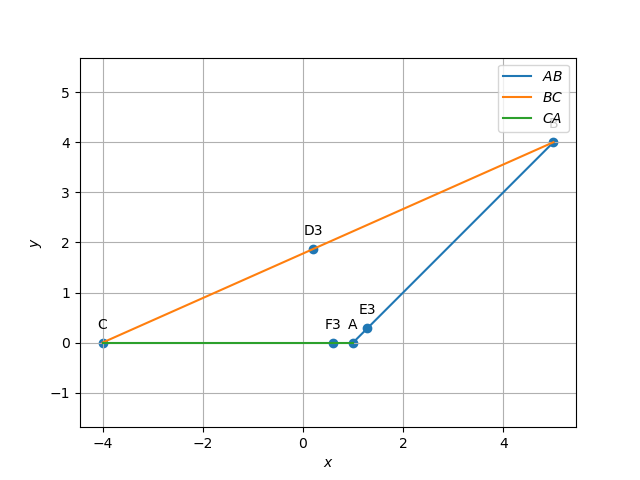
\includegraphics[width=\columnwidth]{/sdcard/digital-design/geometry/figs/points.png}
\caption{Points $D3,E3,F3$}
\label{fig:fig1}
\end{figure}
\item Find the circumcentre and circumradius of $\triangle D_3E_3F_3$.  These are the {\em incentre} and {\em inradius} of $\triangle ABC$. \\
\solution Given 
\begin{align}
    \vec{D}_3 &= \myvec{0.1998795  \\ 1.86661311} \\
    \vec{E}_3 &= \myvec{1.28566988  \\ 0.28566988} \\
    \vec{F}_3 &= \myvec{0.59600178  \\ 0} 
\end{align}
\begin{enumerate}
\item For circumcentre \\
Vector equation of $\vec{D}-\vec{E}$ is
\begin{align}
	(\vec{D}_3-\vec{E}_3)^\top\brak{ \vec{x} - \frac{\vec{D}_3+\vec{E}_3}{2}} = 0 \\
(\vec{D}_3-\vec{F}_3)^\top\brak{ \vec{x} - \frac{\vec{D}_3+\vec{F}_3}{2}} = 0
\end{align}
on Substituting the values of $\vec{D}_3, \vec{E}_3, \vec{F}_3$ and solving We get,
\begin{align}
     \myvec{-1.08579038 & 1.58094323}\vec{x} &= 0.8894235909 \label{eq:1.5.3.6} \\
     \myvec{-0.39612228 & 1.86661311}\vec{x} &= 1.584489107 \label{eq:1.5.3.7}
\end{align}
Thus on solving \eqref{eq:1.5.3.6} and \eqref{eq:1.5.3.7} using gauss elimination We get
\begin{align}
    \myvec{ -1.08579038 & 1.58094323 & 0.8894235909 \\ -0.39612228 & 1.86661311 & 1.584489107} \\
    \therefore \myvec{1&0\\0&1}\vec{x} &= \myvec{0.59600178 \\ 0.97533799}\\
\implies \vec{x}&=\myvec{0.59600178 \\ 0.97533799}
\end{align}
\item The circiumradius is obtained from  $ r=\norm{\vec{I}-\vec{D}_3}$
   \begin{align}
       \vec{I} &= \myvec{0.59600178 \\ 0.97533799} \\
       \vec{D}_3 &= \myvec{0.1998795  \\ 1.86661311} \\
       \vec{I - D_3} &= \myvec{0.39612228 \\-0.89127512} \\
 r= \norm{\vec{I}-\vec{D}_3}\ &=  \sqrt{\brak{\vec{I}-\vec{D}_3}^{\top}\brak{\vec{I}-\vec{D}_3}} \\
 r &= 0.9753379911888156
   \end{align}
\end{enumerate}
\begin{figure}[H]
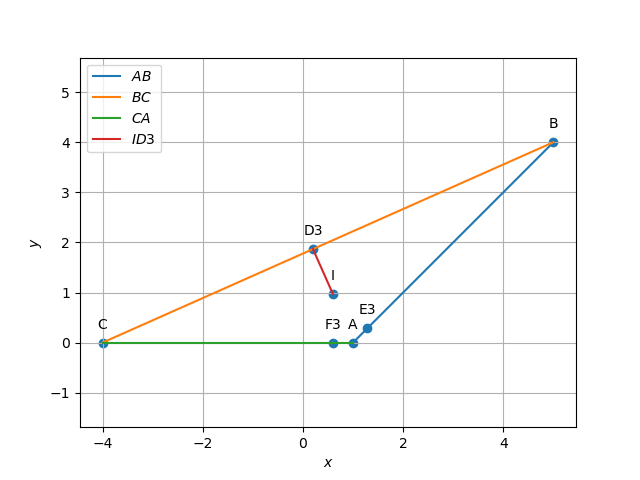
\includegraphics[width=\columnwidth]{/sdcard/digital-design/geometry/figs/Incentre.png}
\caption{Incentre and Inradius of $\triangle ABC$}
\label{fig:fig2}
\end{figure}

 %Question 1.1.4
\item Draw the circumcircle of $\triangle D_3E_3F_3$.  This is known as the {\em incircle} of $\triangle ABC$. \\
\solution 
\begin{align}
    \vec{D}_3 &= \myvec{0.1998795  \\ 1.86661311} \\
    \vec{E}_3 &= \myvec{1.28566988  \\ 0.28566988} \\
    \vec{F}_3 &= \myvec{0.59600178  \\ 0}\\
\text{Incentre}\\ 
    \vec{I} &= \myvec{0.59600178 \\ 0.97533799} \\
\text{Radius}\\
 \vec{r} &=  0.9753379911888156
\end{align}
\begin{figure}[H]
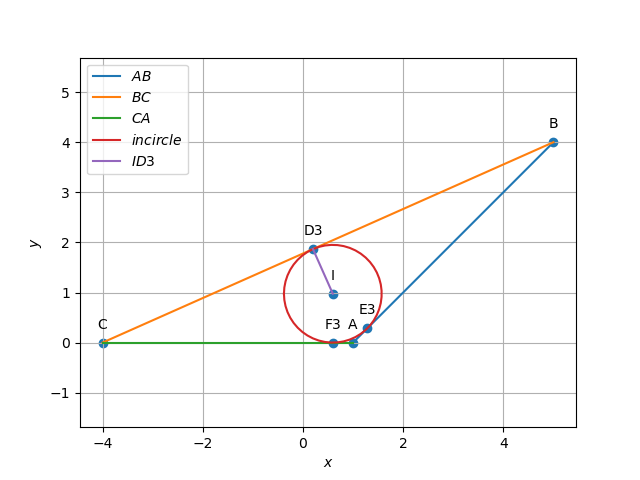
\includegraphics[width=\columnwidth]{/sdcard/digital-design/geometry/figs/incircle.png}
\caption{Incircle of $\triangle ABC$}
\label{fig:fig3}
\end{figure}
  
 %Question 1.1.5
\item Using (1.1.7) verify that 
\begin{align}
\angle BAI = \angle CAI.
\end{align}
$AI$ is the bisector of $\angle A$. \\
\solution
\begin{align}
\label{eq:1.5.5.2}
\cos{\angle BAI} \triangleq \frac{(\vec{B}-\vec{A})\top(\vec{I}-\vec{A})}{\norm{\vec{B}-\vec{A}}\norm{\vec{I}-\vec{A}}} \\
\cos{\angle CAI} \triangleq \frac{(\vec{C}-\vec{A})\top(\vec{I}-\vec{A})}{\norm{\vec{C}-\vec{A}}\norm{\vec{I}-\vec{A}}} 
\end{align}
From the given values of $\vec{A},\vec{B},\vec{C}$ and $\vec{I}$,
\begin{align}
	\vec{B}-\vec{A} &=\myvec{4\\4} \\
	\vec{C}-\vec{A}&= \myvec{-5\\0} \\
 \vec{I}-\vec{A}  &=\myvec{-0.40399822 \\ 0.97533799}
\end{align}
also calculating the values of norms
\begin{align}
	\norm{\vec{B}-\vec{A}} &= \sqrt{32} \\
	\norm{\vec{C}-\vec{A}} &= 5 \\
 	\norm{\vec{I}-\vec{A}} &=  0.8877326906\\
\end{align}
\begin{enumerate}
    \item for $\angle BAI$: \\
    On substtuting the values in  \eqref{eq:1.5.5.2} ,We get 
    \begin{align}
	    \cos{\angle BAI} \triangleq \frac{\myvec{ 4 & 4}\myvec{-0.40399822 \\ 0.97533799}}{ 5.656854249\times 0.8877326906 } \\
    \end{align}
    On solving 
    \begin{align}
        \angle BAI = 62.92928\degree
    \end{align}
       \item for $\angle CAI$: \\
    On substtuting the values in  \eqref{eq:1.5.5.2} ,We get 
    \begin{align}
        \cos{\angle CAI} \triangleq \frac{\myvec{ -5 & 0}\myvec{-0.40399822 \\ 0.97533799}}{5\times 0.8877326906} \\
    \end{align}
    On solving 
    \begin{align}
        \angle CAI = 62.92928\degree
    \end{align}
\end{enumerate}
Therefore $\angle BAI = \angle CAI.$ and $AI$ is the bisector of $\angle A$. 
\begin{figure}[H]
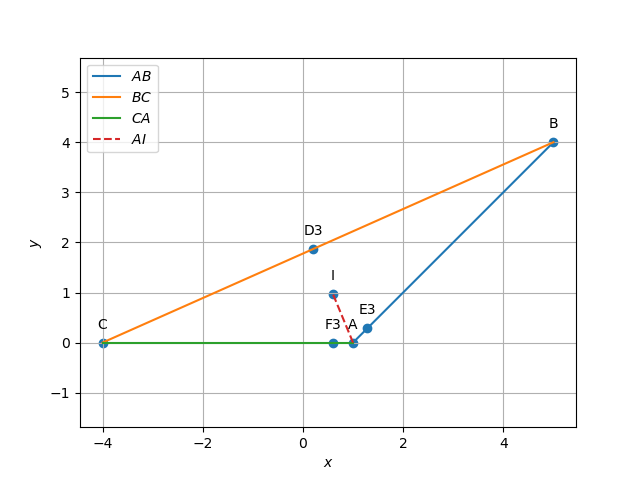
\includegraphics[width=\columnwidth]{/sdcard/digital-design/geometry/figs/AI.png}
\caption{Angular bisector $AI$}
\label{fig:fig4}
\end{figure}

%Question 1.1.6
\item Verify that $BI, CI$ are also the angle bisectors of $\triangle ABC$. \\
\solution
\begin{enumerate}
    \item To prove $BI$ is an angular bisector of $ \angle B$
\begin{align}
\label{eq:1.5.6.1}
\cos{\angle ABI} \triangleq \frac{(\vec{A}-\vec{B})\top(\vec{I}-\vec{B})}{\norm{\vec{A}-\vec{B}}\norm{\vec{I}-\vec{B}}} \\
\cos{\angle CBI} \triangleq \frac{(\vec{C}-\vec{B})\top(\vec{I}-\vec{B})}{\norm{\vec{C}-\vec{B}}\norm{\vec{I}-\vec{B}}} 
\end{align}
From the given values of $\vec{A},\vec{B},\vec{C} and \vec{I}$,\\
\begin{align}
	\vec{A}-\vec{B} &=\myvec{-4\\-4} \\
	\vec{C}-\vec{B}&= \myvec{-9\\-4} \\
 \vec{I}-\vec{B}  &=\myvec{-4.40399822 \\ -3.02466201}
\end{align}
also calculating the values of norms
\begin{align}
	\norm{\vec{A}-\vec{B}} &= \sqrt{32}\\
	\norm{\vec{C}-\vec{B}} &= \sqrt{97} \\
 	\norm{\vec{I}-\vec{B}} &= 5.342637981 \\
\end{align}


\begin{enumerate}
    \item for $\angle ABI$: \\
    On substtuting the values in  \eqref{eq:1.5.6.1} ,We get 
    \begin{align}
        \cos{\angle ABI} \triangleq \frac{\myvec{ -4 & -4}\myvec{-4.40399822 \\ -3.02466201}}{ 5.656854249\times5.342637981} \\
    \end{align}
    On solving 
    \begin{align}
        \angle ABI = 10.5194\degree
    \end{align}
    
       \item for $\angle CBI$: \\
    On substtuting the values in  \eqref{eq:1.5.6.1} ,We get 
    \begin{align}
        \cos{\angle CBI} \triangleq \frac{\myvec{ -9 & -4}\myvec{-4.40399822 \\ -3.02466201}}{ \sqrt{97} \times 5.342637981} \\
    \end{align}
    On solving 
    \begin{align}
        \angle CBI = 10.5194\degree
    \end{align}
    Therefore $\angle ABI = \angle CBI.$ and $BI$ is the bisector of $\angle B$. 
\end{enumerate}

    \item To prove $CI$ is an angular bisector of $ \angle C$
\begin{align}
\label{eq:1.5.6.18}
\cos{\angle BCI} \triangleq \frac{(\vec{B}-\vec{C})\top(\vec{I}-\vec{C})}{\norm{\vec{B}-\vec{C}}\norm{\vec{I}-\vec{C}}} \\
\cos{\angle ACI} \triangleq \frac{(\vec{A}-\vec{C})\top(\vec{I}-\vec{C})}{\norm{\vec{A}-\vec{B}}\norm{\vec{I}-\vec{C}}} 
\end{align}
From the given values of $\vec{A},\vec{B},\vec{C} and \vec{I}$,\\
\begin{align}
	\vec{B}-\vec{C} &=\myvec{9\\4} \\
	\vec{A}-\vec{C}&= \myvec{5\\0} \\
 \vec{I}-\vec{C}  &=\myvec{4.5960178 \\ 0.97533799}
\end{align}
also calculating the values of norms
\begin{align}
	\norm{\vec{B}-\vec{C}} &=\sqrt{97} \\
	\norm{\vec{A}-\vec{C}} &= 5 \\
 	\norm{\vec{I}-\vec{C}} &= 4.698368207 \\
\end{align}

\begin{enumerate}
    \item for $\angle BCI$: \\
    On substtuting the values in  \eqref{eq:1.5.6.18} ,We get 
    \begin{align}
        \cos{\angle BCI} \triangleq \frac{\myvec{ 9 & 4}\myvec{4.5960178 \\ 0.97533799}}{ \sqrt{97}\times 4.698368207} \\
    \end{align}
    On solving 
    \begin{align}
        \angle BCI = 11.98120388 \degree
    \end{align}
       \item for $\angle ACI$: \\
    On substtuting the values in  \eqref{eq:1.5.6.18} ,We get 
    \begin{align}
        \cos{\angle ACI} \triangleq \frac{\myvec{ 5 & 0}\myvec{4.5960178 \\ 0.97533799}}{ 5 \times 4.698368207} \\
    \end{align}
    On solving 
    \begin{align}
        \angle ACI = 11.98120388 \degree
    \end{align}
    Therefore $\angle BCI = \angle ACI.$ and $CI$ is the bisector of $\angle C$. 
\end{enumerate}
\begin{figure}[H]
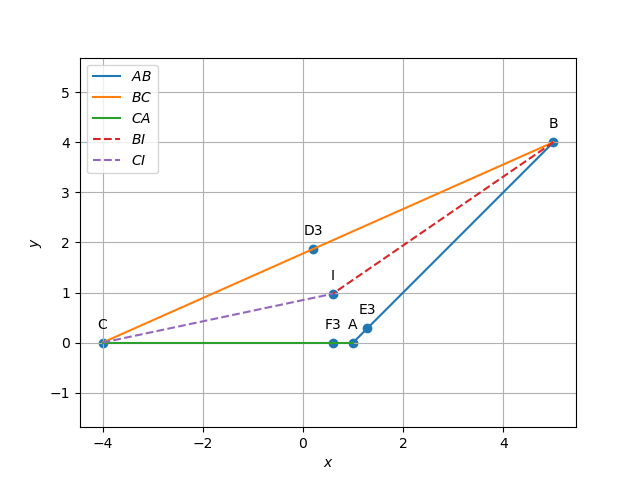
\includegraphics[width=\columnwidth]{/sdcard/digital-design/geometry/figs/BICI.png}
\caption{Angular bisectors  $BI, CI$}
\label{fig:fig5}
\end{figure}
\end{enumerate}

\end{enumerate}
\end{document}
